\section{Galactic Anatomy}
\begin{center} 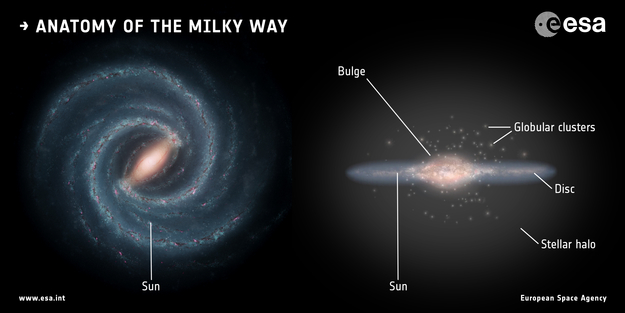
\includegraphics[scale=2]{galaxies/anatomy/pic} \end{center}
\begin{enumerate}
	\item the \textbf{bulge} is the huge, tightly packed group of stars found at the center of a spiral galaxy and as part of lenticular galaxies. there are generally considered to be 2 distinct kinds of bulges.
		\begin{enumerate}
			\item \textbf{classical bulges} have properties similar to elliptical galaxies.
				\begin{itemize}[noitemsep]
					\item comprised of older, redder, Population II stars.
					\item take on a spherical form due to composite stars having orbits which are random in comparison to the plane of the galaxy.
					\item no dust or gas $\rightarrow$ no star formation.
					\item the distribution of light is described by a Sersic profile.
					\item thought to be the results of smaller structures colliding, major mergers make gas clouds more likely to convert to stars.
					\item competing gravitational forces disrupt star orbit paths $\rightarrow$ random orbits.
					\item 80\% of galaxies lack a classical bulge, indicating they have never experienced a major merger.
					\item $\frac{2}{3}$ of galaxies in dense galaxy clusters possess a classical bulge, which demonstrates the disruptive effect of their crowding.
				\end{itemize}
			\item \textbf{disk-like bulges} have properties similar to the central regions of spiral galaxies. often referred to as pseudobulges or disky-bulges.
				\begin{itemize}[noitemsep]
					\item the stars orbit in an ordered fashion in the same plane as the stars in the outer disk.
					\item these bulges have varied structures similar in appearance to spiral galaxies, but 2-100 times smaller.
					\item the rate at which new stars are formed in these bulges is similar to the rate at which stars form in disc galaxies. bulges may contain nuclear rings that are forming stars at much higher rate (per area) than is typically found in outer disks.
					\item theories regarding their formation are uncertain.
						\begin{itemize}[noitemsep]
							\item may be the result of gas-rich mergers which happened more recently (last 5 billion years) than classical bulges, but it is difficult for disks to survive mergers, making this doubtful.
							\item disk galaxies can rearrange their stars and gas in response to instabilities (secular evolution). this process is believed to send gas and dust to the center of a galaxy, increasing the density and creating a bulge.
						\end{itemize}
				\end{itemize}
			\item most bulges and pseudo-bulges are thought to host a central relativistic compact mass, which is traditionally assumed to be a supermassive black hole.
				\begin{itemize}[noitemsep]
					\item  masses of the black holes correlate tightly with bulge properties.
					\item M-sigma relation relates black hole mass to the velocity dispersion of bulge stars
					\item total stellar mass
					\item luminosity
					\item central concentration of stars
					\item  richness of the globular cluster system orbiting in the galaxy's far outskirts
					\item angle of spiral arms
				\end{itemize}
		\end{enumerate}
	\item the \textbf{disc} is a component of disc galaxies (spiral and lenticular). discs consist of 2 components. they tend to be flat, since the orbits of their components tend to be focused in 1 plane, with little vertical motion.
		\begin{enumerate}
			\item the \textbf{stellar component} is composed of most of the galaxy's stars.
				\begin{itemize}[noitemsep]
					\item tends to exhibit little random motions; stars undergo mostly circular orbits around the center.
					\item this leads to the formation of spiral arms in spiral galaxies.
				\end{itemize}
			\item the \textbf{gaseous component} is composed mostly of cool gas and dust.
				\begin{itemize}[noitemsep]
					\item majority of the gaseous component is cool atomic hydrogen (HI) and warm atomic hydrogen (HII). hydrogen is distributed fairly uniformly throughout the disc.
					\item gas serves as fuel for the formation of new stars in the disc.
					\item 21-cm emission by HI shows that the gaseous component can flare at the outer region of the galaxy.
					\item clumps or clouds of gas follow approximately circular orbits about the galactic center.
					\item circular velocity of the gas in the disc is strongly correlated with the luminosity of the galaxy (see Tully-Fisher Relation).
				\end{itemize}
		\end{enumerate}
	\item the \textbf{halo} is an extended, roughly spherical component of a galaxy which extends beyond the main, visible component. The distinction between the halo and the main body of the galaxy is clearest in spiral galaxies, where the spherical shape of the halo contrasts with the flat disc. In an elliptic al galaxy, there is no sharp transition between the other components of the galaxy and the halo.
		\begin{enumerate}
			\item the \textbf{stellar halo} is the component of the halo containing the stars.
				\begin{itemize}[noitemsep]
					\item typically contains oldest, most metal stars.
					\item since they are so faint, studying stellar halos requires very long exposure times.
					\item data from many galaxies must be combined to derive the average properties of a stellar halo. it is only possible to measure individual stars in the Andromeda and Milky Way galaxies.
					\item the furthest stellar halos detected are at a redshift distance of 1.
					\item it is thought that stellar halos consist both of natively created stars and stars obtained from satellite galaxies which merged. this results in streams of stars which are coherent in space or velocity due to being from the same galaxy, as well as variations in properties like metallicity across the halo as a whole.
					\item it is thought that the Milky Way's stellar halo contains 0.1-1\% of its stellar mass.
				\end{itemize}
			\item the \textbf{galactic corona} is the hot, ionized, gaseous component of the galactic halo.
				\begin{itemize}[noitemsep]
					\item coronal gas may be sustained by the \textbf{galactic fountain} --- superbubbles of ionized gas from supernova remnants expands vertically through galactic chimneys into the halo.
					\item as the gas cools, it is eventually pulled back into the disc.
				\end{itemize}
			\item the \textbf{dark matter halo} is a hypothetical part of a galaxy which envelops the galactic disc and extends beyond the edge of the visible galaxy.
				\begin{itemize}[noitemsep]
					\item the presence of dark matter is inferred from its gravitational effect.
						\begin{itemize}[noitemsep]
							\item w/o large amounts of mass throughout the halo, the rotational velocity of the galaxy would decrease the farther it is from the galactic center
							\item however, the rotation curve of most spiral galaxies flattens out.
							\item the absence of visible matter to account for this implies that unobserved, i.e. dark, matter causes it (or that general relativity is incomplete).
						\end{itemize}
					\item dark matter halos are believed to have played a large role in the formation of the early universe.
						\begin{itemize}[noitemsep]
							\item during initial formation, the temperature of the baryonic matter should have still been too high for it to form gravitationally-bound objects alone $\rightarrow$ dark matter structures must have added additional gravitational force b/c dark matter is cold compared to baryonic matter.
							\item hypothesis for CDM structure formation begins with density perturbations in the Universe that grow linearly until they reach a critical density, after which they would stop expanding and collapse to form gravitationally bound dark matter halos. These halos would continue to grow in mass (and size), either through accretion of material from their immediate neighborhood, or by merging with other halos.
						\end{itemize}
				\end{itemize}
		\end{enumerate}
\end{enumerate}
\section{Properties of Galaxies}
\subsection{History}
derived from the Greek \emph{galaxias}, meaning milky.
\subsection{Galaxy Morphological Classification}
astronomers divide galaxies into groups based on their visual appearance. the most often used is the \textbf{Hubble sequence}, invented by Edwin Hubble in 1926. 

\begin{center} 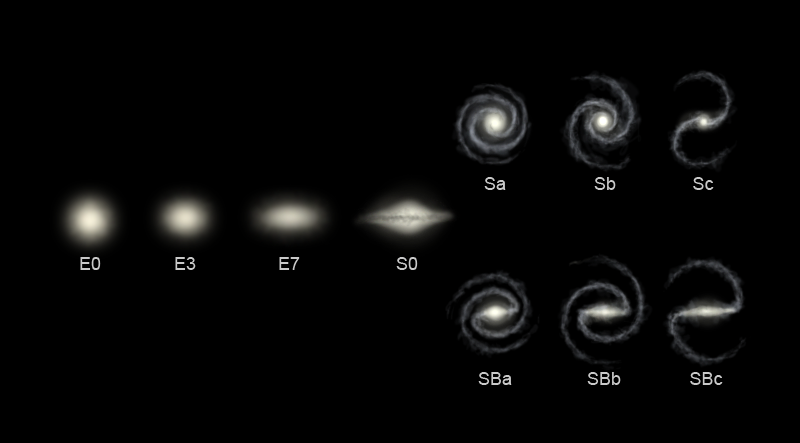
\includegraphics[scale=0.4]{galaxies/fork} \end{center}
\subsubsection{Elliptical Galaxies}
\begin{longtabu} to \textwidth{| | p{3.5cm} | X | |}
\hline
	General Characteristics &
	\begin{itemize}[noitemsep]
		\item smooth, featureless image comprised of ovoid masses of stars attached by the gravitational attraction b/w them
		\item no rotational axis --- stars show wide range of orbital paths around center, primarily radial motion; slight uniformity is what determines overall shape of the galaxy
	\end{itemize}
	\\
	\hline
	Stars &
	\begin{itemize}[noitemsep]
		\item ellipticals contain mostly \textbf{old stars}
			\begin{itemize}[noitemsep]
				\item more red in color
				\item very little gas and dust hampers formation of new stars
			\end{itemize}
	\end{itemize}
	\\
	\hline
	Shapes and Sizes &
	\begin{itemize}[noitemsep]
		\item highest variability of all galaxy types:
			\begin{itemize}[noitemsep]
				\item wide range of masses --- $10^{5}$ to $10^{13}$ solar masses
				\item wide range of sizes --- observations showing that objects can have diameters of between 1 and 100 kiloparsecs (or 3260 to 326,000 light years)
				\item wide range of brightnesses --- some can be up to 10 times brighter than the brightest spirals. At the other end of the scale, the faintest ellipticals can be 1000 times less luminous than the faintest spirals
			\end{itemize}
		\item The Hubble classification of elliptical galaxies contains an integer, $n$ that describes how elongated the galaxy image is. The classification is determined by the ratio of the major (a) to the minor (b) axes of the galaxy's \gls{isophote}s: $ 10 \times (1 - \frac{b}{a}) $
		\item thus, a given elliptical galaxy can be classified as $E_{n}$, where an $E_0$ galaxy is spherical, and an $E_7$ galaxy is flat. this classification is dependent on the angle from which the galaxy is viewed and thus does not affect its physical properties, but is useful for describing how a galaxy appears through a telescope.
	\end{itemize}
	\\
	\hline
	Evolution &
	\begin{itemize}[noitemsep]
		\item astronomers believe that elliptical galaxies form earlier than spiral galaxies, but they can still have quantities of gas and dust, and can still be very noisy in the radio spectrum. evidence has shown that a reasonable proportion (~25\%) of early-type (E, ES and S0) galaxies have residual gas reservoirs and low level star-formation.
		\item evolve from the fusion of smaller, gravitationally bound galaxies which are of similar size
		\item more commonly found around clusters and groups of galaxies due to forming from fusion. They are less frequently spotted in the early universe, which supports the idea that they evolved from the collisions that came later in the life of a galaxy.
		\item A supermassive black hole is thought to lie at the center of these ancient galaxies. These gluttonous giants consume gas and dust, and may play a role in the slower growth of elliptical galaxies.
	\end{itemize}
	\\
	\hline
\end{longtabu}

\subsubsection{Dwarf Elliptical Galaxy}
\begin{longtabu} to \textwidth{| | p{3.5 cm} | X | | }
\hline
General Characteristics &
 elliptical galaxies that are smaller than ordinary elliptical galaxies. They are quite common in galaxy groups and clusters, and are usually companions to other galaxies. Low-luminosity elliptical galaxies are distinguished from late-type galaxies (spirals and irregulars) by their smooth surface-brightness profiles.
Despite their name, dwarf ellipticals are not really fainter versions of true elliptical galaxies, but are structurally distinct.
 \\
 \hline
 Shapes and Sizes &
 Dwarf elliptical galaxies have blue absolute magnitudes within the range ?18 mag < M < ?14 mag, fainter than ordinary elliptical galaxies. Below luminosities of MB approx -18 the smooth-profile galaxies divide into two classes: compact galaxies with high central surface brightnesses (exemplified by M32), and diffuse galaxies with low central surface brightnesses (exemplified by the Local Group dwarf spheroidals).
 
 Typical dE's have masses of about one billion solar masses, or about 1/1000th that of a typical giant galaxy. They contain very little or no gas, which makes them different from dwarf irregular galaxies. Three relatively bright dE's are known in the Local Group: NGC 147, 185, and NGC 205, all companions of the Andromeda Galaxy. Hundreds of similar galaxies exist in the relatively nearby Virgo Cluster.
 \\
 \hline
 Evolution &
 \begin{itemize}[noitemsep]
 	\item thought to be primordial objects built from the coalescing of dark matter and gas objects to form the building blocks of ordinary galaxies
	\item alternately, they could be the remains of low-mass spiral galaxies that were transfigured into a rounder shape through repeated \gls{galaxy harassment}* from ordinary galaxies within a cluster. vidence for the hypothesis had been claimed by studying early-type dwarf galaxies in the Virgo Cluster and finding structures, such as disks and spiral arms, which suggest they are former disk systems transformed by the above-mentioned interactions. However, the existence of similar structures in isolated early-type dwarf galaxies, such as LEDA 2108986, has undermined this hypothesis.
\end{itemize}
\\
\hline
\end{longtabu}
\pagebreak
\subsubsection{Spiral Galaxies}
\begin{longtabu} to \textwidth{| | p{4cm} | X | |}
\hline
	General Characteristics &
	Most spiral galaxies consist of a flat, rotating disk containing stars, gas and dust, and a central concentration of stars known as the bulge. These are often surrounded by a much fainter halo of stars, many of which reside in \gls{globular cluster}s*. Together with irregular galaxies, spiral galaxies make up approximately 60\% of galaxies in today's universe. They are mostly found in low-density regions and are rare in the centers of galaxy clusters.
	\\
	\hline
	Shapes and Sizes &
	\begin{itemize}[noitemsep]
		\item Each spiral galaxy is classified with a label which gives some indication of its appearance:
			\begin{itemize}[noitemsep]
				\item \textbf{$S_{a}$} --- tightly wound spiral arms w/ large central nuclei. 
				\item \textbf{$S_{b}$} --- looser bound spiral arms w/ smaller central nuclei. the majority of spiral galaxies are of type $S_{b}$.
				\item \textbf{$S_{c}$} --- very open, ``untidy" spiral arms and relatively small nuclei. often referred to as the ``grand design."
				
				\begin{center} 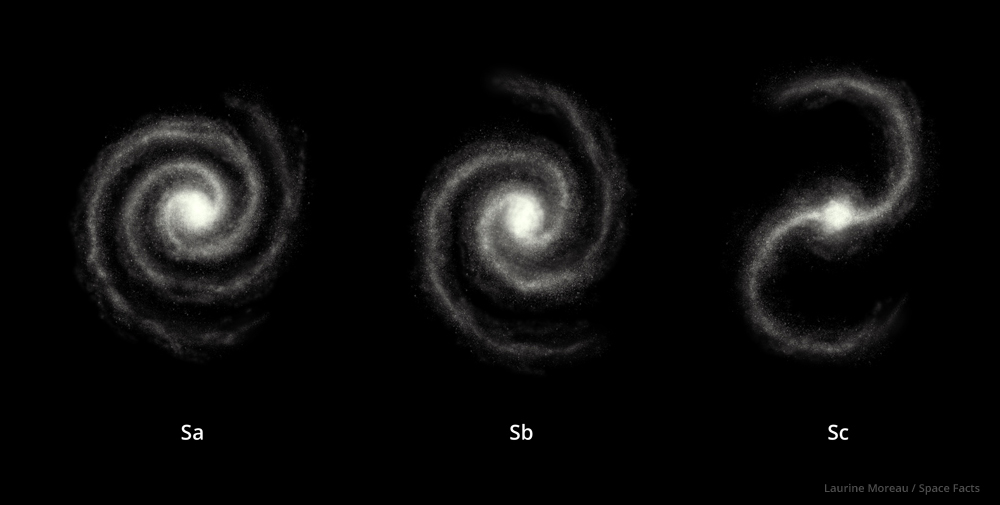
\includegraphics[scale=0.25]{galaxies/spiral/spiral-galaxies} \end{center}
			\end{itemize}
		\item $\frac{2}{3}$ spirals have an additional bar-like elongation of stars extending from the central bulge at the ends of which the spiral arms begin
			\begin{itemize}[noitemsep]
				\item the proportion of barred galaxies has changed over the history of the universe from 10\% to the current amt
				\item these are denoted by the additional label $SB$
				\begin{center} 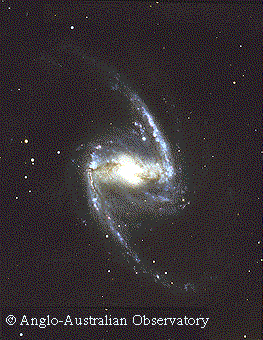
\includegraphics[scale=0.5]{galaxies/spiral/bar} \end{center}
			\end{itemize}
		\item \textbf{bulge} --- a huge, tightly packed central group of stars, often defined as the excess of stellar light above the inward extrapolation of the outer (exponential) disk light. Many bulges are thought to host a supermassive black hole at their centers.
	\end{itemize}
	\\
	\hline
	Celestial Bodies &
	\begin{itemize}[noitemsep]
		\item  The spiral arms are sites of ongoing star formation and are brighter than the surrounding disc because of the young, hot OB stars that inhabit them. Along with fully formed stars, we find sites of stellar formation, with hot glowing clouds of gas and dust forming the ``stellar nurseries" which we see as nebulae in our own galaxy.
			\begin{itemize}[noitemsep]
				\item $S_c$ spirals have the highest proportions of gas and dust, some of which is heated by stars to form nebulae
			\end{itemize}
		\item Using the Hubble classification, the bulge of $S_a$ galaxies is usually composed of Population II stars, that are old, red stars with low metal content. Further, the bulge of Sa and SBa galaxies tends to be large. In contrast, the bulges of $S_c$ and $SB_c$ galaxies are much smaller and are composed of young, blue Population I stars. Some bulges have similar properties to those of elliptical galaxies (scaled down to lower mass and luminosity); others simply appear as higher density centers of disks, with properties similar to disk galaxies.
		\item most stars are located close to the \gls{galactic plane} in conventional circular orbit around the center of the galaxy in a spheroidal bulge around the core
		\item however, some stars inhabit a \textbf{spheroidal halo/galactic spheroid}, a type of galactic halo. The orbital behavior of these stars is disputed, but they may describe retrograde and/or highly inclined orbits, or not move in regular orbits at all. Halo stars may be acquired from small galaxies which fall into and merge with the spiral galaxy.
			\begin{itemize}[noitemsep]
				\item Unlike the galactic disc, the halo seems to be free of dust, and in further contrast, stars in the galactic halo are of Population II, much older and with much lower metallicity than their Population I cousins in the galactic disc (but similar to those in the galactic bulge). The galactic halo also contains many globular clusters.
				\item The motion of halo stars does bring them through the disc on occasion, and a number of small red dwarfs close to the Sun are thought to belong to the galactic halo, and due to their irregular movement around the center of the galaxy, these stars often display unusually high proper motion.
			\end{itemize}
	\end{itemize}
	\\
	\hline
	Evolution &
	\begin{itemize}[noitemsep]
		\item the most prominent theory regarding the formation of the spiral arms is the \textbf{density wave theory} --- stars move thru intermittent periods of great density as part of their orbital cycle which form spiral shapes
			\begin{itemize}[noitemsep]
				\item the density wave rotates slower than the material in the galactic disc, so that stars and gas are able to ``overtake" the wave
				\item as interstellar gas passes thru the density wave, it becomes more dense, leading to the formation of new stars
				\item the hottest stars live for a very short time, so they appear bright within the spiral arms during their lifetime, but as they pass out of the spirals and into the galactic disk, they die and become dim, explaining the contrast in brightness
			\end{itemize}
		\item the older stars of the bulge and halo are thought to have formed through the primordial collapse of individual gas clouds early in the history of the Universe
			\begin{itemize}[noitemsep]
				\item bulges, especially those of $S_c$ and $S_d$ type galaxies, sometimes contain younger stars; after the spiral bulges of these galaxies had formed through primordial collapse, they also experienced some form of secular evolution --- through accretion processes or the actions of spiral arms or a central bar
			\end{itemize}
		\item disks are thought to form after the primordial collapse event responsible for the formation of the spheroidal bulge and halo, possibly through the cooling of the hot gas contained within the halo of the newly formed galaxy. however, spiral galaxies have both thick disks (composed entirely of stars) and thin disks (also containing cold gas).
			\begin{itemize}[noitemsep]
				\item on average, the thick disk is older than the thin disk but younger than the bulge. It has therefore been suggested that the thick disk may have formed through a significant merger event early in the Galaxy?s history. Both observations and N-body modelling indicate that such an event would disrupt the thin disk and consume a significant fraction of the cold gas in a burst of new star formation, so the proposed merger event must have taken place before the thin disk had time to fully form.
				\item An alternative to this major merger scenario is one in which the thick disk formed relatively slowly through the actions of multiple minor mergers. Once the merger events had formed the thick disk, the stars retained the scale height of the thick disk while the cold gas collapsed back into the galactic plane to form the thin disk.
				\item ongoing star formation takes place in the thin disk. This star formation is usually on the leading edge of the spiral arms where the cold gas of the thin disk is compressed.
			\end{itemize}
	\end{itemize}
	\\
	\hline
\end{longtabu}
			
\pagebreak
\subsubsection{Lenticular Galaxies}
\begin{longtabu} to \textwidth{| | p{4cm} | X | |}
\hline
	General Characteristics &
	a type of galaxy intermediate between an elliptical (denoted E) and a spiral galaxy in galaxy morphological classification schemes, they are also known as $S_0$ galaxies. they contain large discs but do not have large spiral arms; they are disc galaxies that have used up or lost most of their interstellar matter and therefore have very little ongoing star formation. however, they retain significant dust in their disks. As a result, they consist mainly of aging stars (like elliptical galaxies). 
	\\
	\hline
	Shapes and Sizes &
	\begin{itemize}[noitemsep]
		\item visible disk component w/ large bulge 
		\item much higher bulge-to-disk ratios than typical spirals
		\item may exhibit central bar
		\item lenticular galaxies can be classified according to the $S0_n$ and $SB0_n$ systems
			\begin{itemize}[noitemsep]
				\item in the $S0_n$ system, $n$ indicates the amount of dust present
				\item in the $SB0_n$ system, $n$ indicates the prominence of the bar. $SB0_1$ galaxies have the least defined bar structure and are only classified as having slightly enhanced surface brightness along opposite sides of the central bulge. The prominence of the bar increases with index number, thus $SB0_3$ galaxies have very well defined bars that can extend through the transition region between the bulge and disk.
			\end{itemize}
	\end{itemize}
	\\
	\hline
	Celestial Bodies &
	In many respects the composition of lenticular galaxies is like that of ellipticals. For example, they both consist of predominately older, hence redder, stars. All of their stars are thought to be older than about a billion years, in agreement with their offset from the Tully?Fisher relation. In addition to these general stellar attributes, globular clusters* are found more frequently in lenticular galaxies than in spiral galaxies of similar mass and luminosity. They also have little to no molecular gas (hence the lack of star formation) and no significant hydrogen $\alpha$ or 21-cm emission. Finally, unlike ellipticals, they may still possess significant dust.
	\\
	\hline
	Evolution & 
	\begin{enumerate}
		\item The absence of gas, presence of dust, lack of recent star formation, and rotational support are all attributes one might expect of a spiral galaxy which had used up all of its gas in the formation of stars
			\begin{enumerate}
				\item anemic* spiral galaxies are similar to lenticular galaxies if the spiral pattern were dispersed
				\item according to the Tully-Fisher relation, spiral galaxies and lenticular galaxies have the same slope on the luminosity/absolute magnitude axis, but are offset by $\Delta I = 1.5$. This implies that lenticular galaxies were once spiral galaxies but are now dominated by old, red stars.
			\end{enumerate}
		\item it has also been postulated that lenticular galaxies form from galaxy mergers.
			\begin{enumerate}
				\item  lenticular galaxies typically have surface brightness much greater than other spiral classes. It is also thought that lenticular galaxies exhibit a larger bulge-to-disk ratio than spiral galaxies and this may be inconsistent with simple fading from a spiral. they also have an increased frequency of globular clusters*.
				\item Mergers are unable to account for the offset from the Tully?Fisher relation without assuming that the merged galaxies were quite different from those we see today.
				\item advanced models of the central bulge indicate that it is smaller, lessening the inconsistency.
			\end{enumerate}
	\end{enumerate}
	\\
	\hline
\end{longtabu}
	
	
\pagebreak
\section{Globular Clusters}
\subsection{Composition}
\begin{itemize}[noitemsep]
	\item a spherical collection of stars orbiting a galactic core as a satellite
	\item the force of gravity maintains the spherical shape and gives them a high stellar density towards their center
	\item hundreds of thousands of old, low-metal stars --- there is no gas or dust, implying it was all turned into stars
		\begin{itemize}[noitemsep]
			\item Globular clusters can contain a high density of stars; on average about 0.4 stars per cubic parsec, increasing to 100 or 1000 stars per cubic parsec in the core of the cluster. The typical distance between stars in a globular cluster is about 1 light year.
			\item normally Population II stars w/ low proportion of elements other than hydrogen or helium (i.e. low metallicity)
			\item \textbf{Oosterhoff groups} --- 2 populations of globular clusters
				\begin{itemize}[noitemsep]
					\item group 1 --- ``metal-rich," has a slightly stronger metallic spectral line
					\item group 2 --- ``metal-poor," has a slightly weaker metallic spectral line w/ a slightly longer period of RR Lyrae variable stars
					\item  Many scenarios have been suggested to explain these subpopulations, including violent gas-rich galaxy mergers, the accretion of dwarf galaxies, and multiple phases of star formation in a single galaxy. In the Milky Way, the metal-poor clusters are associated with the halo and the metal-rich clusters with the bulge.
				\end{itemize}
		\end{itemize}
	\item the high star density leads to close interactions and near-collisions of stars often $\rightarrow$ exotic classes of stars are very common in globular clusters
		\begin{itemize}[noitemsep]
			\item e.g.  blue stragglers, millisecond pulsars and low-mass X-ray binaries
			\item searches for black holes in the center of globular clusters have demonstrated evidence for a new kind of black hole intermediate b/w the standard black hole and the supermassive. the mass of these intermediate black holes is proportionate the mass of the clusters.
			\item however, this is disputed b/c the heaviest objects in globular clusters will migrate to the center due to the effects \gls{mass segregation}*. therefore, the sharp increase in mass-to-light ratio toward the center of a cluster may be possible without the presence of a black hole.
		\end{itemize}
\end{itemize}
\subsection{Formation}
\begin{itemize}[noitemsep]
	\item  it remains uncertain whether the stars in a globular cluster form in a single generation or are spawned across multiple generations over a period of several hundred million years
	\item  In many globular clusters, most of the stars are at approximately the same stage in stellar evolution, suggesting that they formed at about the same time. However, the star formation history varies from cluster to cluster, with some clusters showing distinct populations of stars.
	\item it is also theorized that globular clusters w/ variation in their star populations formed from the merging of multiple clusters, which is consistent w/ Hubble Telescope Observations of massive clusters of clusters in close proximity
	\item clusters typically arise in regions of efficient star formation w/ interstellar medium of a higher density than in normal star-forming regions
	\item Research indicates a correlation between the mass of a central supermassive black holes (SMBH) and the extent of the globular cluster systems of elliptical and lenticular galaxies. The mass of the SMBH in such a galaxy is often close to the combined mass of the galaxy's globular clusters.
	\item No known globular clusters display active star formation, which is consistent with the view that globular clusters are typically the oldest objects in the Galaxy, and were among the first collections of stars to form. Very large regions of star formation known as super star clusters, such as Westerlund 1 in the Milky Way, may be the precursors of globular clusters.
\end{itemize}
\pagebreak
\section{The Tully-Fisher Relation}
\begin{itemize}[noitemsep]
	\item an empirical relationship between the mass or intrinsic luminosity of a spiral galaxy and its angular velocity or emission line width,  first published in 1977 by astronomers R. Brent Tully and J. Richard Fisher.
	\item  The luminosity is calculated by multiplying the galaxy's apparent brightness/magnitude by $4\pi d^2$, where d is its distance from us, and the spectral-line width is measured using long-slit spectroscopy.
	\item everal different forms of the TFR exist, depending on which precise measures of mass, luminosity or rotation velocity one takes it to relate. Tully and Fisher used optical luminosity, but subsequent work showed the relation to be tighter when defined using microwave to infrared (K band) radiation (a good proxy for stellar mass), and even tighter when luminosity is replaced by the galaxy's total baryonic mass (the sum of its mass in stars and gas). This latter form of the relation is known as the Baryonic Tully?Fisher relation (BTFR), and states that baryonic mass is proportional to velocity to the power of roughly 3.5?4.
	\item The TFR can be used to estimate the distance to spiral galaxies by allowing the luminosity of a galaxy to be derived from its directly measurable line width. The distance can then be found by comparing the luminosity to the apparent brightness. Thus the TFR constitutes a rung of the cosmic distance ladder, where it is calibrated using more direct distance measurement techniques and used in turn to calibrate methods extending to larger distance.
	\item In the dark matter p*aradigm, a galaxy's rotation velocity (and hence line width) is primarily determined by the mass of the dark matter halo in which it lives, making the TFR a manifestation of the connection between visible and dark matter mass. In Modified Newtonian Dynamics (MOND), the BTFR (with power-law index exactly 4) is a direct consequence of the gravitational force law effective at low acceleration.
	\item The analogues of the TFR for non-rotationally-supported galaxies, such as ellipticals, are known as the Faber-Jackson relation and the Fundamental Plane.
\end{itemize}

		
